\section{设计挑战：性能、状态、一致性与安全}
\label{sec:challenges}

Agent框架从第一代工具链到第五代自主Agent的每一次代际跃迁，都暴露了新的系统性问题——这些问题既不能靠模型本身解决，也不能靠临时性的工程修补来根治。
本节以统一的框架审视五个横切设计挑战：（1）~用具体场景描述问题；（2）~分析根本原因；（3）~梳理当前解决方案；（4）~与经典计算机体系结构中已被充分研究的问题进行显式类比。
在全文中，我们将每个挑战追溯到ICA层次（第~\ref{sec:icam}节）和定量定律（第~\ref{sec:laws}节），论证第~\ref{sec:framework}节引入的双平面架构不仅仅是组织上的便利，而是对这些挑战的\emph{必要的}结构性回应。


%% ---------- 延迟与吞吐 ----------
\subsection{延迟、吞吐与成本的三元约束}

\subsubsection{场景}
假设一个代码Agent正在帮助开发者修复一个跨10个文件的bug。
Agent需要阅读多个文件（每次阅读触发模型推理）、理解代码结构、定位问题、修改代码、运行测试、查看结果、再修改。
整个流程可能涉及20--50次模型调用，每次调用的延迟直接影响开发者的等待时间。
如果单次调用延迟是2秒，总延迟可能超过1分钟。
如果服务提供商为了降低延迟而增加GPU并行度，每次调用的成本会显著上升。
反之，如果提供商通过增大批处理规模来摊薄成本、提高吞吐，单个请求的排队时间就会拉长，延迟随之上升。
这就是\emph{延迟--吞吐--成本三元约束}：降低延迟需要更多资源（增加成本），提高吞吐需要更大的批处理（增加延迟），控制成本需要更少的资源（同时增加延迟和降低吞吐）。

\subsubsection{根因}
大模型推理的解码阶段存在一个经典的结构性矛盾。
\textbf{预填充}（prefill）阶段是\emph{计算密集型}的：需要处理整个输入序列，GPU的计算单元满负荷工作，瓶颈在FLOPS。
\textbf{解码}（decode）阶段是\emph{内存带宽密集型}的：每生成一个新token，都需要读取全部模型权重和当前KV缓存——这本质上是"每个时钟周期都要从内存搬移一遍参数"\cite{gholami2024memorywall}。
Gholami等人量化了这一结构性失衡：峰值FLOPS以每两年$3.0\times$的速度增长，而DRAM带宽仅以每两年$1.6\times$的速度增长\cite{gholami2024memorywall}。

由于两个阶段对硬件资源的需求根本不同，将它们混合在同一个批处理中必然导致某种资源利用不足：预填充阶段独占计算资源，解码阶段则在等待内存带宽。
Agent工作负载进一步加剧了这一问题：多个子Agent并发发起请求，请求之间的上下文长度差异巨大（有的只读一个函数，有的需要理解整个仓库），这使得静态批处理策略效率低下。

\subsubsection{当前方案}
研究社区从多个层面应对这一约束。

\paragraph{调度层优化。}
ORCA\cite{orca2022}提出迭代级调度（iteration-level scheduling）：不等待整个序列生成完毕再调度新请求，而是每个解码步结束后检查是否可以加入新请求，显著提高了GPU利用率。
DistServe\cite{zhong2024distserve}将预填充和解码彻底分离到不同的GPU组，使每组可以独立优化：预填充组用高FLOPS的GPU，解码组用高内存带宽的GPU。
Sarathi-Serve\cite{agrawal2024sarathi}引入了stall-free调度：通过chunked prefill将长输入切分为固定大小的块，与解码任务混合调度，消除了解码阶段因等待大型预填充而产生的停顿。

\paragraph{内存管理优化。}
vLLM\cite{kwon2023pagedattention,vllm_docs_2026}通过PagedAttention将KV缓存组织为固定大小的页，通过block table映射到非连续物理空间，实现了KV缓存的按需分配和共享。
SGLang\cite{sglang2024,sglang_docs_2026}通过RadixAttention将请求前缀组织为基数树（radix tree），自动识别和复用共享前缀的KV缓存。
TGI\cite{tgi_docs_2026}和TensorRT-LLM\cite{tensorrtllm_docs_2026}则在工业级部署中实现了连续批处理和页式KV管理。
vAttention\cite{prabhu2024vattention}提供了另一种思路：利用OS级别的连续虚拟内存和动态增长，直接支持标准注意力内核，避免了对PagedAttention专用内核的依赖。

图~\ref{fig_trilemma}展示了三方权衡关系。三个目标中任意两个可以联合优化，但同时改善全部三个目标在结构上不可行。
\begin{figure}[htbp]
    \centering
    \begin{tikzpicture}[scale=1.05]
    
    % ── Triangle vertices ─────────────────────────────────────────────────────────
    \coordinate (A) at (0,   3.5);   % top: Low Latency
    \coordinate (B) at (-3.0, 0);    % bottom-left: Low Cost
    \coordinate (C) at ( 3.0, 0);    % bottom-right: High Throughput
    
    % ── Fill triangle lightly ────────────────────────────────────────────────────
    \fill[gray!8] (A) -- (B) -- (C) -- cycle;
    \draw[gray!40, thick] (A) -- (B) -- (C) -- cycle;
    
    % ── Vertex labels ────────────────────────────────────────────────────────────
    \node[font=\small\bfseries, text=classical!80!black, align=center] at (0, 4.15)
        {Low Latency\\{\scriptsize (fast response)}};
    
    \node[font=\small\bfseries, text=modelnative!80!black, align=center] at (-3.8, -0.55)
        {Low Cost\\{\scriptsize (efficient resource)}};
    
    \node[font=\small\bfseries, text=black!70, align=center] at (3.8, -0.55)
        {High Throughput\\{\scriptsize (batch efficiency)}};
    
    % ── Edge annotations (outside triangle edges, not overlapping) ───────────────
    \node[font=\scriptsize, text=gray!55, rotate=54, align=center]
        at (-2.2, 2.0) {small batch,\\dedicated GPU};
    
    \node[font=\scriptsize, text=gray!55, rotate=-54, align=center]
        at (2.2, 2.0) {more GPUs,\\higher cost};
    
    \node[font=\scriptsize, text=gray!55, align=center]
        at (0, -0.35) {large batch, queue longer};
    
    % ── "Pick any two" label in centre ──────────────────────────────────────────

    
    % ── System design example points ─────────────────────────────────────────────
    % Interactive agent: low latency + low cost side
    % 【修改点】：将文字的 X 坐标从 -0.8 改为 -0.6，使其向右平移一点点
    \filldraw[classical!70] (-0.8, 1.8) circle (3.5pt);
    \node[font=\scriptsize, text=classical!80, anchor=north] at (-0.6, 1.65)
        {Interactive agent};
    
    % Batch pipeline: high throughput + low cost side
    \filldraw[modelnative!70] (1.2, 0.6) circle (3.5pt);
    \node[font=\scriptsize, text=modelnative!80, anchor=east] at (1.0, 0.6)
        {Batch pipeline};
    
    % RT serving: low latency + high throughput
    \filldraw[black!55] (0.5, 2.5) circle (3.5pt);
    \node[font=\scriptsize, text=black!65, anchor=east] at (0.3, 2.5)
        {RT serving};
    
    % ── Classical analogy note (no citation) ─────────────────────────────────────
    \node[font=\scriptsize, text=gray!50, align=center] at (0, -1.4)
        {Classical analogy: response time -- throughput trade-off in time-sharing OS};
    
    \end{tikzpicture}
    \caption{The latency--throughput--cost trilemma in LLM serving. Any two objectives can be jointly optimised, but improving all three simultaneously is structurally infeasible given the compute-bound prefill / bandwidth-bound decode asymmetry. Representative system designs are plotted as points inside the triangle.}
    \label{fig_trilemma}
    \end{figure}

\subsubsection{经典类比}
这组问题与经典计算机体系结构中的\emph{内存墙}（Memory Wall）问题直接对应。
1980年代以来，CPU速度以每年约50\%的速度增长，而DRAM延迟仅以每年约7\%的速度改善\cite{hennessy2017quantitative}。
体系结构的应对——多级缓存（L1/L2/L3）、硬件预取和写缓冲——直接映射到LLM推理中的KV缓存分层、前缀缓存和异步解码。
分时操作系统中的"响应时间--吞吐量"权衡也与此对应：交互式任务需要低响应时间（低延迟），批处理任务需要高吞吐量（大batch），调度器需要在两者之间寻找平衡点\cite{ostep_2023}。

在ICA中，这一三元约束主要跨越L1（物理执行）和L2（推理服务）。
定律I（第~\ref{sec:law1}节）量化了这一权衡的缓存侧：KV缓存命中率$H$直接决定了可达到的加速比，任何调度或内存管理优化都可以理解为在三元约束下最大化$H$的尝试。


%% ---------- 状态管理 ----------
\subsection{状态管理与跨会话一致性}

\subsubsection{场景}
假设一个用户连续三天使用同一个Agent来开发一个项目。
第一天，Agent学会了用户偏好"使用TypeScript而不是JavaScript"。
第二天，用户要求Agent重构代码，Agent需要在遵循第一天学到的偏好的同时，正确理解代码的当前状态。
第三天，用户发现了一个新bug，Agent需要回忆前两天做过哪些修改（因为bug可能是前两天引入的），同时理解项目的最新状态。
更进一步，如果用户在第二天同时运行了两个Agent实例（一个做重构，一个写测试），两个Agent可能同时修改同一个文件，产生冲突。

\subsubsection{根因}
传统CPU是\emph{无状态}执行器：给定相同的输入和寄存器状态，输出是确定且可重复的。
智能系统则必须跨会话\emph{持久化}状态：用户偏好（"我喜欢TypeScript"）、历史任务记录（"昨天我们重构了认证模块"）、以及外部世界变化（"代码仓库新增了三个文件"）。
一旦引入持久状态，至少三类问题必然出现：

\begin{enumerate}[nosep]
\item \textbf{多Agent共享记忆的并发访问。}
当多个Agent同时读写共享记忆时，如何保证一致性？
这类似于多线程编程中的竞态条件。

\item \textbf{延迟提交与冲突合并。}
Agent~A修改了文件但尚未提交；Agent~B基于旧版本开始修改同一文件。
检测和解决此类冲突类似于分布式系统中的乐观并发控制。

\item \textbf{记忆时效性。}
三天前学到的"项目使用React"可能已经过时（项目迁移到了Vue）。
判断记忆是否仍然有效类似于缓存失效（cache invalidation）问题。
\end{enumerate}

\subsubsection{当前方案}
LongMemEval\cite{longmemeval2024}的评估说明，长期记忆并不是简单地"存更多聊天记录"，而是涉及四种能力：信息抽取（从对话中提取关键事实）、时序推理（理解事件的先后顺序）、知识更新（当新信息与旧记忆冲突时更新记忆）、和拒答能力（当记忆不足以支持回答时主动拒绝）。

MemGPT\cite{memgpt2023}借鉴了OS虚拟内存的分页和换入换出机制来管理上下文，将上下文分为"主存"（当前活跃的对话窗口）和"外存"（向量数据库中的长期记忆），通过编辑和检索操作在两者之间移动信息。
MemoryOS\cite{memoryos2025}将记忆管理抽象为操作系统的内存管理模块，实现了结构化的记忆编码、检索和更新。
A-MEM\cite{amem2025}提出了Agent式的记忆管理：记忆不再是被动存储的字符串，而是由Agent自主决定何时写入、何时更新、何时删除的"活跃实体"。
Letta\cite{letta_stateful_2026}（前身为MemGPT项目）进一步将"有状态Agent"作为核心抽象，显式区分了对话状态、核心记忆和归档记忆。

从分布式系统角度看，至少需要区分三种状态类型\cite{raft2014,spanner2012,cap2002}：
\begin{enumerate}[nosep]
\item \textbf{局部可丢弃状态}（ephemeral state）：当前推理步骤的中间结果，类似于CPU寄存器，不需要持久化。
\item \textbf{需因果有序的会话状态}（session state）：同一任务内Agent间的消息传递和状态传递，类似于分布式系统中的因果一致性保证\cite{raft2014}。
\item \textbf{需要强可追溯和可回放的提交状态}（committed state）：对文件、数据库或外部系统的永久修改，类似于数据库事务的commit point，需要支持审计和回滚\cite{spanner2012}。
\end{enumerate}

图~\ref{fig:state_lifecycle}展示了这三种状态类型的生命周期及其与ICA层的映射。
% ---------------------------------------------------------------------------
% Agent State Lifecycle — three-tier state classification
% fig:state_lifecycle
% ---------------------------------------------------------------------------
\begin{figure}[htbp]
\centering
\providecolor{ephColor}{HTML}{4A78A8}
\providecolor{sessColor}{HTML}{E07B39}
\providecolor{commColor}{HTML}{3A8A3A}
\providecolor{timeColor}{HTML}{888888}
%
\resizebox{0.90\textwidth}{!}{%
\begin{tikzpicture}[
    font=\small, >=Latex,
    statebox/.style={draw=#1!70!black, fill=#1!15, rounded corners=5pt,
        minimum width=3.8cm, minimum height=1.1cm,
        align=center, font=\small\bfseries, text=#1!85!black, line width=0.7pt},
    opbox/.style={draw=#1!50, fill=#1!8, rounded corners=3pt,
        minimum width=3.4cm, minimum height=0.65cm,
        align=center, font=\scriptsize, text=#1!70!black, line width=0.4pt},
    analogbox/.style={draw=gray!40, fill=gray!6, rounded corners=3pt,
        minimum width=3.4cm, minimum height=0.65cm,
        align=center, font=\scriptsize, text=gray!65!black, line width=0.4pt},
    arrowstyle/.style={-{Latex[length=2mm]}, thick, line width=0.65pt},
    timelabel/.style={font=\scriptsize, text=timeColor!80},
]

% ============================================================
% STATE 1: Ephemeral
% ============================================================
\node[statebox=ephColor] (E) at (-4.8, 2.2)
    {Ephemeral State};
\node[opbox=ephColor] at (-4.8, 1.15)  {Scope: single inference step};
\node[opbox=ephColor] at (-4.8, 0.30)  {Persistence: none required};
\node[analogbox]      at (-4.8, -0.65) {Analogy: CPU registers};
\node[opbox=ephColor] at (-4.8, -1.65) {Examples: KV activations,\\intermediate logits};

% ============================================================
% STATE 2: Session
% ============================================================
\node[statebox=sessColor] (S) at (0.5, 2.2)
    {Session State};
\node[opbox=sessColor] at (0.5, 1.15)  {Scope: within-task agent chain};
\node[opbox=sessColor] at (0.5, 0.30)  {Consistency: causal ordering};
\node[analogbox]      at (0.5, -0.65) {Analogy: distributed message\\passing (Raft)};
\node[opbox=sessColor] at (0.5, -1.65) {Examples: agent handoff state,\\intermediate results};


% ============================================================
% STATE 3: Committed
% ============================================================
\node[statebox=commColor] (C) at (5.5, 2.2)
    {Committed State};
\node[opbox=commColor] at (5.5, 1.15)  {Scope: permanent side effects};
\node[opbox=commColor] at (5.5, 0.30)  {Consistency: full auditability};
\node[analogbox]       at (5.5, -0.65) {Analogy: DB transaction\\commit (Spanner)};
\node[opbox=commColor] at (5.5, -1.65) {Examples: file writes, DB\\updates, code commits};


% ============================================================
% ICA layer labels
% ============================================================
\node[font=\scriptsize\bfseries, ephColor!80!black, anchor=north] at (-4.8, -2.2)
    {ICA L2 (KV cache)};
\node[font=\scriptsize\bfseries, sessColor!80!black, anchor=north] at (0.5, -2.2)
    {ICA L3--L5 (context / orch.)};
\node[font=\scriptsize\bfseries, commColor!80!black, anchor=north] at (5.5, -2.2)
    {ICA L4--L6 (interface / app)};

% lifetime bars (moved up)
\fill[ephColor!30] (-6.5,-3.2) rectangle (-2.0,-2.8);
\node[font=\tiny, text=ephColor!80] at (-4.25, -3.0) {ephemeral lifetime};

\fill[sessColor!30] (-2.0,-3.2) rectangle (2.5,-2.8);
\node[font=\tiny, text=sessColor!80] at (0.25, -3.0) {session lifetime};

\fill[commColor!30] (2.5,-3.2) rectangle (7.0,-2.8);
\node[font=\tiny, text=commColor!80] at (4.75, -3.0) {committed lifetime};

% timeline (moved up)
\draw[{Latex[length=2.5mm]}-, thick, timeColor!50, line width=1.0pt]
    (-6.5, -3.5) -- (7.2, -3.5);
\node[timelabel, anchor=west] at (7.3, -3.5) {time};
\foreach \x/\lbl in {-6.0/Step start, -2.0/Task boundary, 2.5/Commit point, 6.5/Session end}{
    \draw[timeColor!40, line width=0.5pt] (\x, -3.35) -- (\x, -3.65);
    \node[timelabel, anchor=north] at (\x, -3.7) {\lbl};
}

% ============================================================
% State transition arrows
% ============================================================
\draw[arrowstyle, ephColor!60]
    (E.north east) -- ++(0, 0.45) -|
    node[above, font=\scriptsize, text=black!50, pos=0.35] {promote on task boundary}
    (S.north west);
\draw[arrowstyle, sessColor!60]
    (S.north east) -- ++(0, 0.45) -|
    node[above, font=\scriptsize, text=black!50, pos=0.35] {commit on side-effect}
    (C.north west);

% Rollback arrow — routed above all boxes
\draw[arrowstyle, commColor!50, dashed, rounded corners=4pt]
    (C.north) -- ++(0, 1.2)
    -- ++(-5.0, 0)
    node[above, midway, font=\scriptsize, text=black!45] {rollback on failure}
    -- (S.north);

\end{tikzpicture}}%
\caption{Three-tier agent state lifecycle. \textbf{Ephemeral state} (left) lives only within a single inference step and requires no persistence, analogous to CPU registers. \textbf{Session state} (centre) spans an agent task chain and requires causal consistency guarantees, analogous to distributed message passing. \textbf{Committed state} (right) constitutes permanent, auditable side effects and requires full rollback support, analogous to a database transaction commit. Arrows indicate promotion on task boundaries and rollback paths on failure.}
\label{fig:state_lifecycle}
\end{figure}


\subsubsection{长时运行Agent的时序衰减}
值得特别关注的是，Agent执行的时间跨度正在从分钟级向小时乃至天级扩展。
最新的工业实践表明，Agent已能自主运行超过7小时完成复杂任务\cite{anthropic2026agenticreport}。
这种跨小时乃至跨天的持续执行引入了额外的时序衰减挑战：注意力衰减函数$\beta(L)$不再仅仅是上下文位置的函数，还与会话持续时间和跨步骤的状态积累有关。
这意味着上述三种状态类型的划分需要增加一个时间维度：跨小时执行需要KV缓存的会话持久化（L2），上下文窗口管理需要支持跨检查点的工作集恢复（L3），治理层需要定义定期检查点与人工恢复协议（L5）。
定律II（第~\ref{sec:law2}节）当前的模型尚未捕捉这一时序维度，这是后续研究的重要方向。

\subsubsection{经典类比}
这组问题对应经典计算机中的\emph{虚拟内存与分布式一致性}。
OS的虚拟内存通过页表将虚拟地址映射到物理地址，并提供换入换出机制来制造"内存无限大"的幻觉——对应Agent系统的上下文管理。
分布式文件系统（如GFS/Spanner\cite{spanner2012}）通过Paxos/Raft\cite{raft2014}共识协议保证多副本的一致性——对应多Agent共享记忆的一致性。
CAP定理\cite{cap2002}指出一致性、可用性和分区容错性三者不可兼得；Agent系统的记忆管理同样面临这一权衡：是选择强一致性（每次操作都等待所有副本同步）还是最终一致性（允许短暂的不一致以换取低延迟）。

在ICA中，这一挑战主要跨越L3（上下文管理）和L5（编排）。
双平面架构自然地将问题分离：概率执行平面管理工作上下文（记住什么、遗忘什么），确定性控制平面则执行一致性保证和冲突解决协议。


%% ---------- 接口漂移 ----------
\subsection{接口漂移与版本兼容}

\subsubsection{场景}
一个Agent被配置为使用GitHub API来管理代码仓库。
某天GitHub更新了API，将\texttt{repos/:owner/:repo/pulls}的返回格式从v3改为v4，新增了分页参数，删除了部分字段。
Agent的工具调用开始返回错误或解析失败。
更隐蔽的情况：Agent使用的提示模板依赖模型产生特定格式的输出（如"always respond in JSON"），但模型升级后输出风格发生了微妙变化，导致下游解析器频繁崩溃。
类似的问题还出现在MCP服务器更新能力描述、技能包接口变更、以及记忆文件格式版本升级等场景。

\subsubsection{根因}
传统计算机系统之所以可扩展，很大程度上源于其核心接口——包括ISA、ABI、系统调用和文件格式——\emph{数十年来保持稳定}。
x86指令集从1978年的8086到2026年的最新处理器，核心指令集保持了向后兼容；POSIX标准自1988年确立以来，\texttt{read()}/\texttt{write()}/\texttt{fork()}等系统调用的语义几乎没有变化\cite{ostep_2023}。
这种稳定性使得上层软件可以安心构建，而不必担心底层接口突然变化。

相比之下，当前Agent生态存在严重的\emph{接口漂移}（interface drift）。
漂移的来源至少有四种：
\begin{enumerate}[nosep]
\item \textbf{模型版本漂移：}模型升级后，对相同提示的输出格式可能变化。
\item \textbf{工具schema漂移：}外部API的接口描述和返回格式可能随时更新\cite{mcp_intro_2026}。
\item \textbf{协议漂移：}MCP、A2A等协议本身还在快速迭代\cite{agentprotocols2025,google_a2a_2025}。
\item \textbf{技能包漂移：}可复用的Agent技能在不同项目或不同模型版本上的表现可能不同。
\end{enumerate}

\subsubsection{当前方案}
OpenAI Codex通过AGENTS.md\cite{openai_codex_agents_md_2026}和Skills\cite{openai_codex_skills_2026}机制提供了项目级的接口稳定锚点：技能包有明确的版本号和兼容性声明。
Claude Code通过CLAUDE.md\cite{anthropic_claudecode_memory_2026}实现类似的功能。
互操作性协议——包括用于模型--工具通信的MCP\cite{mcp_intro_2026}和用于Agent--Agent交互的A2A\cite{google_a2a_2025}——正在尝试建立标准化接口。
A2A协议基于JSON-RPC 2.0 over HTTP，定义了Agent发现、能力协商和任务委派的标准流程\cite{google_a2a_2025}。
然而，这些协议本身也在快速迭代，尚未达到ISA或POSIX那样的稳定性。

\subsubsection{经典类比}
这对应经典计算机中的\emph{ABI稳定性与版本管理}。
Intel维持x86 ISA的向后兼容已经超过45年；Linux内核维持系统调用的向后兼容已经超过30年；甚至共享库的版本管理也有成熟的方案（如semantic versioning和symbol versioning）。
模型原生计算架构需要建立自己的"版本控制学"：工具schema需要版本号，模型输出格式需要兼容性声明，技能包需要依赖管理（类似npm的\texttt{package.json}），记忆文件需要格式迁移工具（类似数据库的schema migration）。

在ICA中，接口漂移主要影响L4（语义接口层）和L4--L5边界。
确定性控制平面必须维护版本感知的接口契约，使概率执行平面与上游变更隔离——这正是ABI稳定性在保护应用软件免受硬件演进影响方面所扮演的角色。


%% ---------- 安全隐私 ----------
\subsection{安全、隐私与最小权限}

\subsubsection{场景}
一个代码Agent正在帮助开发者处理用户数据。
Agent需要读取包含用户隐私的数据库表结构（以理解数据模型）、修改处理用户数据的代码、运行测试（测试数据中可能包含真实用户信息）。
在这个过程中，Agent可能：（1）~将敏感数据写入日志文件或发送到远程API（数据泄露）；（2）~被恶意的代码注释或文件内容通过提示注入劫持，执行非预期的操作（目标劫持）；（3）~在测试中使用真实用户数据而非模拟数据（隐私违规）。
更危险的是：由于Agent可以执行任意shell命令，一个精心构造的提示注入可能让它运行\texttt{rm -rf /}或上传敏感文件到外部服务器。

\subsubsection{根因}
一旦Agent可以读写文件、运行命令、浏览网页、调用数据库，它就不再只是语言模型，而是具备外部行动能力的\emph{主体}（agent in the security sense）。
这带来了传统软件安全无法覆盖的新攻击面：

\begin{enumerate}[nosep]
\item \textbf{提示注入}（prompt injection）。
攻击者通过在工具返回的数据、文件内容或网页中嵌入恶意指令来劫持Agent的行为。
与传统的代码注入（如SQL注入）不同，提示注入利用的不是代码逻辑的缺陷，而是模型无法区分"用户的指令"与"数据中嵌入的指令"\cite{debenedetti2025camel,owasp_agentic2026}。

\item \textbf{权限过度配置}（privilege over-provisioning）。
当前大多数Agent在获得工具访问权限时，获得的是该工具的\emph{全量}权限（如"可以读写整个文件系统"），而不是最小必要权限（如"只能读写项目目录下的特定文件"）。

\item \textbf{记忆污染传播}（memory taint propagation）。
一次成功的提示注入可以将恶意信息写入Agent的长期记忆，这些"被污染"的记忆会在后续所有会话中影响Agent的行为，形成持久的后门\cite{aura2025}。
\end{enumerate}

\subsubsection{当前方案}
工业界和学术界正在从多个维度构建防御体系。

\paragraph{沙箱隔离。}
OpenAI Codex默认在OS强制沙箱内运行，每个任务在独立的容器中执行，无法访问宿主机的文件系统或网络\cite{openai_codex_sandbox_2026}。
Claude Code默认只读模式，任何写操作都需要用户显式授权\cite{anthropic_claudecode_security_2026}。
Aura在移动端为每个App Agent建立独立的沙箱，并限制Agent Kernel对系统资源的访问\cite{aura2025}。

\paragraph{能力安全模型。}
CaMeL\cite{debenedetti2025camel}将操作系统的capability安全原则应用于防御提示注入：Agent不能直接执行有副作用的操作，而是通过一个确定性的capability manager获取"临时通行证"。
每个通行证只授权一个特定操作（如"只读文件\texttt{src/main.py}"），用后即废。
这从根本上消除了"提示注入导致权限提升"的可能，因为权限是由确定性代码而非概率式模型决定的。

\paragraph{审批与审计。}
Codex的approval policies\cite{openai_codex_approvals_2026}允许开发者定义哪些操作需要人工审批（如"任何\texttt{DELETE}操作都需要确认"）。
Agents SDK的tracing机制\cite{openai_codex_agentsdk_2026}记录了每一次工具调用的完整上下文，支持事后审计和回放。

\paragraph{安全形式化。}
IronClaw\cite{ironclaw2025}提出了面向Agent安全的形式化框架，将Agent的行为空间和权限空间显式建模，通过静态分析和运行时监控来检测越界行为。
Christodorescu等人\cite{agenticsecurity2025}进一步论证了Agent安全需要借鉴操作系统安全的全部经验：最小权限、隔离、审计和失败安全（fail-safe defaults）。

\subsubsection{经典类比}
这对应经典计算机中的\emph{进程安全与权限管理}。
Unix的安全模型建立在三个核心概念上：（1）~用户态/内核态分离——用户程序不能直接访问硬件，必须通过系统调用\cite{ostep_2023}；（2）~文件权限（rwx）——每个文件有明确的读、写和执行权限；（3）~root/非root分离——特权操作需要显式权限提升。
Agent安全需要类似的三层模型：（1）~概率平面/确定性平面分离——Agent不能直接执行有副作用的操作，必须通过确定性控制平面的审批通道；（2）~工具capability标注——每个工具有明确的能力声明和权限要求；（3）~治理层权限提升——高风险操作需要显式授权或人工确认。

\subsubsection{双重用途的安全关切}
必须认识到，Agent能力具有固有的双重用途特性。
同样的能力既可以用于自动化安全审计（防御性用途），也可以用于自动化漏洞发现和利用（攻击性用途）\cite{anthropic2026agenticreport}。
这意味着双平面架构的确定性控制平面不仅要约束自身Agent的行为，还必须预判对手也拥有等效的双平面系统。
Anthropic 2026年的Agent安全报告预测"Agent化网络防御系统"将以机器速度运行\cite{anthropic2026agenticreport}，这意味着L5治理层的原语设计必须从一开始就将对抗性场景纳入威胁模型。

在ICA中，安全跨越全部六层，但集中在L4（工具能力标注和调用审计）和L5（权限审批和失败恢复）。
双平面架构在此至关重要：概率平面处理解释用户意图所需的推理能力，确定性平面则执行不可协商的安全不变量。


%% ---------- 治理层 ----------
\subsection{治理：体系结构的第一性重点}

\subsubsection{核心问题}
ArbiterOS\cite{arbiteros2025}指出，Agent工程的根本危机来自一个结构性矛盾：开发者本能地用\emph{确定性软件思维}来驱动一个\emph{概率式处理器}。
传统软件工程中，代码的行为是确定性的：相同的输入必然产生相同的输出，测试可以覆盖所有分支，bug可以通过断言来检测。
Agent的行为则由概率式模型驱动：相同的提示可能产生不同的输出，测试无法覆盖所有可能的推理路径，"bug"以幻觉或指令遵循失败的形式出现，且难以通过传统断言检测。

Aura\cite{aura2025}进一步说明，一旦Agent进入操作系统和移动端环境，权限管理（Agent是否有权访问联系人列表？）、身份验证（调用Agent的是真正的用户还是攻击者？）、语义输入污染（一条恶意短信是否可以劫持Agent？）、以及记忆污染传播（被污染的记忆如何清理？）都会变成\emph{内核级}问题——不再是某个应用的安全漏洞，而是整个系统体系结构的安全基础。

图~\ref{fig:challenge_heatmap}将每个挑战映射到其影响最大的ICA层次，展示了在完整技术栈上的主要、次要和第三级影响。
\begin{figure}[h]
\centering
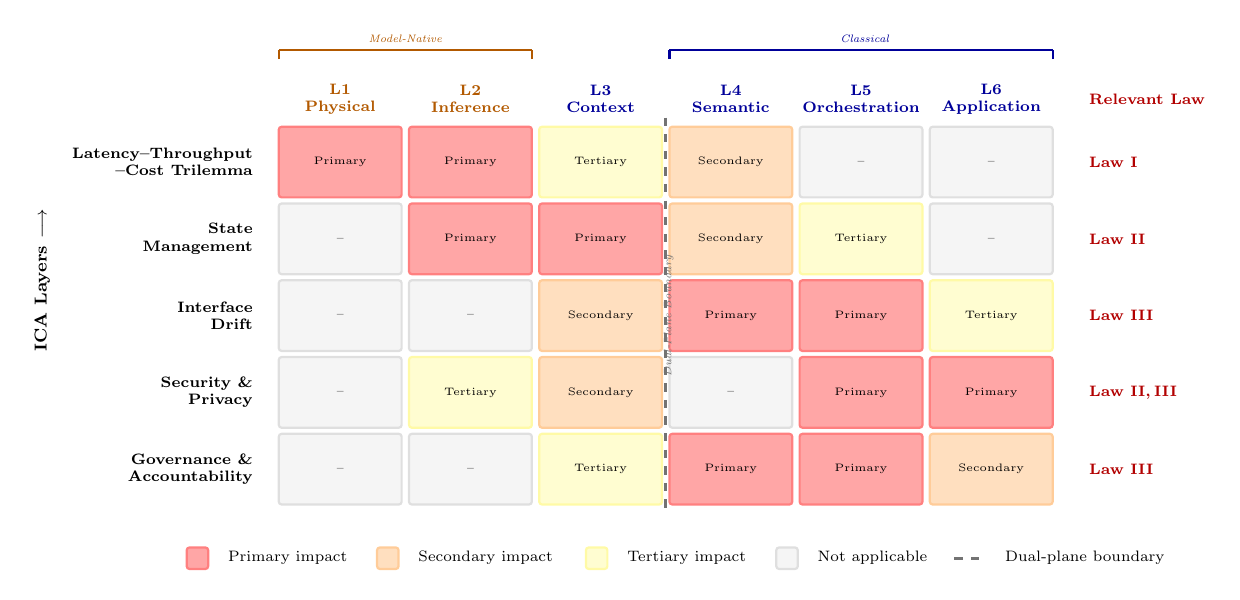
\begin{tikzpicture}[
    scale=0.78,
    transform shape,
    % --- cell styles by severity ---
    primary/.style={fill=red!35, draw=red!50, thick, rounded corners=1pt},
    secondary/.style={fill=orange!25, draw=orange!40, thick, rounded corners=1pt},
    tertiary/.style={fill=yellow!18, draw=yellow!35, thick, rounded corners=1pt},
    notapplic/.style={fill=gray!8, draw=gray!25, thick, rounded corners=1pt},
    % --- header styles ---
    colhead/.style={font=\scriptsize\bfseries, align=center, text width=1.8cm},
    rowhead/.style={font=\scriptsize\bfseries, align=right, anchor=east, text width=3.4cm},
    lawlabel/.style={font=\scriptsize\bfseries, align=center, anchor=west},
    celltxt/.style={font=\tiny, align=center},
    % --- axis labels ---
    axlbl/.style={font=\footnotesize\bfseries},
]

% === dimensions ===
\def\cellw{2.0}   % column width (cm)
\def\cellh{1.15}   % row height (cm)
\def\colsep{0.12}  % horizontal gap between cells
\def\rowsep{0.10}  % vertical gap between cells
\def\rowoff{5}     % number of rows minus 1 (0-indexed)
\def\coloff{5}     % number of cols minus 1 (0-indexed)

% === origin offsets ===
\def\xstart{4.0}   % left edge of first data column
\def\ystart{6.2}    % top edge of first data row

% === column headers (L1--L6) ===
% Use explicit two-line labels to prevent word-break hyphenation
\pgfmathsetmacro{\cx}{\xstart + 0*(\cellw+\colsep) + \cellw/2}
\node[colhead, text=orange!70!black] at (\cx, \ystart + 0.45) {L1\\Physical};
\pgfmathsetmacro{\cx}{\xstart + 1*(\cellw+\colsep) + \cellw/2}
\node[colhead, text=orange!70!black] at (\cx, \ystart + 0.45) {L2\\Inference};
\pgfmathsetmacro{\cx}{\xstart + 2*(\cellw+\colsep) + \cellw/2}
\node[colhead, text=blue!60!black] at (\cx, \ystart + 0.45) {L3\\Context};
\pgfmathsetmacro{\cx}{\xstart + 3*(\cellw+\colsep) + \cellw/2}
\node[colhead, text=blue!60!black] at (\cx, \ystart + 0.45) {L4\\Semantic};
\pgfmathsetmacro{\cx}{\xstart + 4*(\cellw+\colsep) + \cellw/2}
\node[font=\scriptsize\bfseries, align=center, text width=2.2cm, text=blue!60!black] at (\cx, \ystart + 0.45) {L5\\Orchestration};
\pgfmathsetmacro{\cx}{\xstart + 5*(\cellw+\colsep) + \cellw/2}
\node[colhead, text=blue!60!black] at (\cx, \ystart + 0.45) {L6\\Application};

% === column sub-headers: plane labels (raised slightly) ===
\pgfmathsetmacro{\modelnativex}{\xstart + \cellw + \colsep/2}
\node[font=\tiny\itshape, orange!70!black, anchor=south] at (\modelnativex, \ystart + 1.25) {Model-Native};
\pgfmathsetmacro{\classicalx}{\xstart + 3*(\cellw+\colsep) + 1.5*\cellw + 1.5*\colsep}
\node[font=\tiny\itshape, blue!60!black, anchor=south] at (\classicalx, \ystart + 1.25) {Classical};

% === row headers (5 challenges) ===
\pgfmathsetmacro{\rx}{\xstart - 0.3}
\pgfmathsetmacro{\ryA}{\ystart - 0*(\cellh+\rowsep) - \cellh/2}
\pgfmathsetmacro{\ryB}{\ystart - 1*(\cellh+\rowsep) - \cellh/2}
\pgfmathsetmacro{\ryC}{\ystart - 2*(\cellh+\rowsep) - \cellh/2}
\pgfmathsetmacro{\ryD}{\ystart - 3*(\cellh+\rowsep) - \cellh/2}
\pgfmathsetmacro{\ryE}{\ystart - 4*(\cellh+\rowsep) - \cellh/2}
\node[rowhead] at (\rx, \ryA)
    {Latency--Throughput\\--Cost Trilemma};
\node[rowhead] at (\rx, \ryB)
    {State\\Management};
\node[rowhead] at (\rx, \ryC)
    {Interface\\Drift};
\node[rowhead] at (\rx, \ryD)
    {Security \&\\Privacy};
\node[rowhead] at (\rx, \ryE)
    {Governance \&\\Accountability};

% === heatmap cells ===
% Row 0: Latency/Cost -- Primary L1,L2; Secondary L4; Tertiary L3; NA L5,L6
\foreach \c/\sty in {0/primary, 1/primary, 2/tertiary, 3/secondary, 4/notapplic, 5/notapplic}{
    \pgfmathsetmacro{\xll}{\xstart + \c*(\cellw+\colsep)}
    \pgfmathsetmacro{\yll}{\ystart - \cellh}
    \draw[\sty] (\xll, \yll) rectangle +(\cellw, \cellh);
}
% Severity text inside cells
\foreach \c/\lab in {0/Primary, 1/Primary, 2/Tertiary, 3/Secondary, 4/--, 5/--}{
    \pgfmathsetmacro{\cx}{\xstart + \c*(\cellw+\colsep) + \cellw/2}
    \pgfmathsetmacro{\cy}{\ystart - \cellh + \cellh/2}
    \node[celltxt] at (\cx, \cy) {\lab};
}

% Row 1: State Mgmt -- Primary L2,L3; Secondary L4; Tertiary L5; NA L1,L6
\foreach \c/\sty in {0/notapplic, 1/primary, 2/primary, 3/secondary, 4/tertiary, 5/notapplic}{
    \pgfmathsetmacro{\xll}{\xstart + \c*(\cellw+\colsep)}
    \pgfmathsetmacro{\yll}{\ystart - 1*(\cellh+\rowsep) - \cellh}
    \draw[\sty] (\xll, \yll) rectangle +(\cellw, \cellh);
}
\foreach \c/\lab in {0/--, 1/Primary, 2/Primary, 3/Secondary, 4/Tertiary, 5/--}{
    \pgfmathsetmacro{\cx}{\xstart + \c*(\cellw+\colsep) + \cellw/2}
    \pgfmathsetmacro{\cy}{\ystart - 1*(\cellh+\rowsep) - \cellh + \cellh/2}
    \node[celltxt] at (\cx, \cy) {\lab};
}

% Row 2: Interface Drift -- Primary L4,L5; Secondary L3; Tertiary L6; NA L1,L2
\foreach \c/\sty in {0/notapplic, 1/notapplic, 2/secondary, 3/primary, 4/primary, 5/tertiary}{
    \pgfmathsetmacro{\xll}{\xstart + \c*(\cellw+\colsep)}
    \pgfmathsetmacro{\yll}{\ystart - 2*(\cellh+\rowsep) - \cellh}
    \draw[\sty] (\xll, \yll) rectangle +(\cellw, \cellh);
}
\foreach \c/\lab in {0/--, 1/--, 2/Secondary, 3/Primary, 4/Primary, 5/Tertiary}{
    \pgfmathsetmacro{\cx}{\xstart + \c*(\cellw+\colsep) + \cellw/2}
    \pgfmathsetmacro{\cy}{\ystart - 2*(\cellh+\rowsep) - \cellh + \cellh/2}
    \node[celltxt] at (\cx, \cy) {\lab};
}

% Row 3: Security & Privacy -- Primary L5,L6; Secondary L3; Tertiary L2; NA L1,L4
\foreach \c/\sty in {0/notapplic, 1/tertiary, 2/secondary, 3/notapplic, 4/primary, 5/primary}{
    \pgfmathsetmacro{\xll}{\xstart + \c*(\cellw+\colsep)}
    \pgfmathsetmacro{\yll}{\ystart - 3*(\cellh+\rowsep) - \cellh}
    \draw[\sty] (\xll, \yll) rectangle +(\cellw, \cellh);
}
\foreach \c/\lab in {0/--, 1/Tertiary, 2/Secondary, 3/--, 4/Primary, 5/Primary}{
    \pgfmathsetmacro{\cx}{\xstart + \c*(\cellw+\colsep) + \cellw/2}
    \pgfmathsetmacro{\cy}{\ystart - 3*(\cellh+\rowsep) - \cellh + \cellh/2}
    \node[celltxt] at (\cx, \cy) {\lab};
}

% Row 4: Governance -- Primary L4,L5; Secondary L6; Tertiary L3; NA L1,L2
\foreach \c/\sty in {0/notapplic, 1/notapplic, 2/tertiary, 3/primary, 4/primary, 5/secondary}{
    \pgfmathsetmacro{\xll}{\xstart + \c*(\cellw+\colsep)}
    \pgfmathsetmacro{\yll}{\ystart - 4*(\cellh+\rowsep) - \cellh}
    \draw[\sty] (\xll, \yll) rectangle +(\cellw, \cellh);
}
\foreach \c/\lab in {0/--, 1/--, 2/Tertiary, 3/Primary, 4/Primary, 5/Secondary}{
    \pgfmathsetmacro{\cx}{\xstart + \c*(\cellw+\colsep) + \cellw/2}
    \pgfmathsetmacro{\cy}{\ystart - 4*(\cellh+\rowsep) - \cellh + \cellh/2}
    \node[celltxt] at (\cx, \cy) {\lab};
}

% === Dual-plane boundary: thick dashed line between L3 and L4 ===
\pgfmathsetmacro{\bndx}{\xstart + 3*(\cellw+\colsep) - \colsep/2}
\pgfmathsetmacro{\bndtop}{\ystart + 0.15}
\pgfmathsetmacro{\bndbot}{\ystart - 4*(\cellh+\rowsep) - \cellh - 0.15}
\draw[very thick, dashed, black!55] (\bndx, \bndtop) -- (\bndx, \bndbot);

% Small label for the boundary
\pgfmathsetmacro{\bndmid}{(\bndtop + \bndbot)/2}
\node[font=\tiny\itshape, black!55, rotate=90, anchor=south] at (\bndx + 0.25, \bndmid)
    {Dual-Plane Boundary};

% === Right-margin annotation: quantitative law relevance ===
\pgfmathsetmacro{\lawx}{\xstart + 6*(\cellw+\colsep) + 0.35}

% Row 0: Latency/Cost -> Law I (Energy/Performance scaling)
\pgfmathsetmacro{\ry}{\ystart - 0*(\cellh+\rowsep) - \cellh/2}
\node[lawlabel, red!70!black] at (\lawx, \ry) {Law~I};

% Row 1: State Mgmt -> Law II (Memory/State consistency)
\pgfmathsetmacro{\ry}{\ystart - 1*(\cellh+\rowsep) - \cellh/2}
\node[lawlabel, red!70!black] at (\lawx, \ry) {Law~II};

% Row 2: Interface Drift -> Law III (Interface stability)
\pgfmathsetmacro{\ry}{\ystart - 2*(\cellh+\rowsep) - \cellh/2}
\node[lawlabel, red!70!black] at (\lawx, \ry) {Law~III};

% Row 3: Security & Privacy -> Law III + II
\pgfmathsetmacro{\ry}{\ystart - 3*(\cellh+\rowsep) - \cellh/2}
\node[lawlabel, red!70!black] at (\lawx, \ry) {Law~II,\,III};

% Row 4: Governance -> Law III
\pgfmathsetmacro{\ry}{\ystart - 4*(\cellh+\rowsep) - \cellh/2}
\node[lawlabel, red!70!black] at (\lawx, \ry) {Law~III};

% Right-margin column header
\node[font=\scriptsize\bfseries, red!70!black, anchor=west] at (\lawx, \ystart + 0.45)
    {Relevant Law};

% === Axis labels ===
\pgfmathsetmacro{\axleft}{\xstart - 3.6}
\pgfmathsetmacro{\axmid}{\ystart - 2*(\cellh+\rowsep)}
\node[axlbl, rotate=90, anchor=south] at (\axleft, \axmid)
    {ICA Layers $\longrightarrow$};

\pgfmathsetmacro{\axbotx}{\xstart + 2.5*(\cellw+\colsep)}
\pgfmathsetmacro{\axboty}{\ystart - 4*(\cellh+\rowsep) - \cellh - 0.5}
\node[axlbl, anchor=north] at (\axbotx, \axboty) {};

% === Legend (centred, items spaced so text doesn't overlap next box) ===
\def\legy{-1.0}
\def\legx{2.5}
% Each item: box(0.35) + gap(0.2) + text + gap(0.5) before next box
% "Primary impact" ~1.8cm, "Secondary impact" ~2.1cm, "Tertiary impact" ~1.7cm
% item spacing: 3.1cm apart

% Primary
\draw[primary] (\legx, \legy) rectangle +(0.35, 0.35);
\node[font=\scriptsize, anchor=west] at (\legx + 0.55, \legy + 0.175)
    {Primary impact\hspace{0.4em}};

% Secondary  (start at legx + 3.1)
\pgfmathsetmacro{\lx}{\legx + 3.1}
\draw[secondary] (\lx, \legy) rectangle +(0.35, 0.35);
\node[font=\scriptsize, anchor=west] at (\lx + 0.55, \legy + 0.175)
    {Secondary impact\hspace{0.4em}};

% Tertiary  (start at legx + 6.5)
\pgfmathsetmacro{\lx}{\legx + 6.5}
\draw[tertiary] (\lx, \legy) rectangle +(0.35, 0.35);
\node[font=\scriptsize, anchor=west] at (\lx + 0.55, \legy + 0.175)
    {Tertiary impact\hspace{0.4em}};

% Not applicable  (start at legx + 9.6)
\pgfmathsetmacro{\lx}{\legx + 9.6}
\draw[notapplic] (\lx, \legy) rectangle +(0.35, 0.35);
\node[font=\scriptsize, anchor=west] at (\lx + 0.55, \legy + 0.175)
    {Not applicable\hspace{0.4em}};

% Boundary legend entry  (start at legx + 12.5)
\pgfmathsetmacro{\lx}{\legx + 12.5}
\draw[very thick, dashed, black!55] (\lx, \legy + 0.175) -- ++(0.5, 0);
\node[font=\scriptsize, anchor=west] at (\lx + 0.7, \legy + 0.175)
    {Dual-plane boundary};

% Plane annotations along top
\pgfmathsetmacro{\modelleft}{\xstart}
\pgfmathsetmacro{\modelright}{\xstart + 2*\cellw + \colsep}
\pgfmathsetmacro{\classleft}{\xstart + 3*(\cellw+\colsep)}
\pgfmathsetmacro{\classright}{\xstart + 5*(\cellw+\colsep) + \cellw}
\pgfmathsetmacro{\bracetop}{\ystart + 1.1}

% Underbrace for model-native plane
\draw[thick, orange!70!black]
    (\modelleft, \bracetop) -- (\modelleft, \bracetop + 0.15);
\draw[thick, orange!70!black]
    (\modelright, \bracetop) -- (\modelright, \bracetop + 0.15);
\draw[thick, orange!70!black]
    (\modelleft, \bracetop + 0.15) -- (\modelright, \bracetop + 0.15);

% Underbrace for classical plane
\draw[thick, blue!60!black]
    (\classleft, \bracetop) -- (\classleft, \bracetop + 0.15);
\draw[thick, blue!60!black]
    (\classright, \bracetop) -- (\classright, \bracetop + 0.15);
\draw[thick, blue!60!black]
    (\classleft, \bracetop + 0.15) -- (\classright, \bracetop + 0.15);

\end{tikzpicture}
\caption{Challenge-to-ICA-layer impact heatmap. Each cell indicates the severity of a given challenge at the corresponding ICA layer: \textcolor{red!50}{\textbf{primary}} (direct, critical impact), \textcolor{orange!40}{\textbf{secondary}} (significant but indirect), \textcolor{yellow!50!black}{\textbf{tertiary}} (moderate, contextual), or \textcolor{gray!40}{not applicable}. The thick dashed line marks the dual-plane boundary between model-native layers (L1--L2) and classical layers (L3--L6). The right-margin column identifies the most relevant quantitative law for each challenge row.}
\label{fig:challenge_heatmap}
\end{figure}


\subsubsection{治理不是补丁}
上述观察意味着，治理绝不应被当作事后的安全补丁或合规检查清单。
正如操作系统设计者通过数十年的惨痛教训认识到的事后加装安全从根本上不可行\cite{ostep_2023}，Agent系统的治理也必须从第一天就嵌入体系结构之中。

\subsubsection{ICA逐层治理}
具体而言，ICA（第~\ref{sec:icam}节）的每一层都需要对应的治理机制：

\begin{itemize}[nosep]
\item \textbf{L1---物理执行层：}硬件级的推理精度保证和能耗预算。
类似于CPU的温度监控和频率调节，L1需要确保推理精度不低于安全阈值（如量化不能导致关键判断出错），以及GPU/TPU的能耗在可控范围内。

\item \textbf{L2---推理服务层：}推理预算和精度治理。
每个Agent的推理调用应该有预算上限（如"每个子任务最多10次推理调用"），超出预算应触发失败恢复而非无限重试。
KV缓存管理需要保证关键状态不被意外驱逐。

\item \textbf{L3---上下文管理层：}记忆保留和删除策略。
用户的敏感信息（如密码、信用卡号）应有自动检测和及时删除机制（类似于GDPR的"被遗忘权"）。
记忆的时效性应有明确的TTL（time-to-live）标注，过期记忆应自动降级或删除。

\item \textbf{L4---语义接口层：}工具能力标注和调用审计。
每个外部工具应有标准化的能力声明（"这个工具能做什么、不能做什么、有什么副作用"），每次工具调用都应被记录在可审计的trace中。
MCP协议\cite{mcp_intro_2026}正在朝这个方向发展。

\item \textbf{L5---编排层：}权限审批和失败恢复。
高风险操作（写入文件、发送邮件、执行shell命令）应通过确定性控制平面的审批流程。
失败恢复应有明确的回滚策略（如git revert）和人工接管机制。

\item \textbf{L6---应用层：}用户意图确认和副作用声明。
在执行任何不可逆操作前，系统应向用户确认理解正确。
每个用户任务执行完毕后，系统应生成副作用报告（"本次任务修改了哪些文件、发送了哪些邮件、访问了哪些外部服务"）。
\end{itemize}

\subsubsection{双平面架构中的治理}
从第~\ref{sec:framework}节提出的双平面架构视角看，治理层正是确定性控制平面中的\emph{核心组件}。
它的职责不是替代概率平面的推理能力，而是为推理结果设置边界、维护审计轨迹和提供回滚机制。
具体来说：
概率平面负责"理解用户意图、分解任务、生成工具调用参数"——这是LLM擅长的推理能力；
确定性平面负责"检查权限是否满足、工具调用是否安全、结果是否合规、失败是否可恢复"——这是传统软件工程擅长的确定性逻辑。
CaMeL\cite{debenedetti2025camel}的capability manager、Codex\cite{openai_codex_approvals_2026}的approval policies、Claude Code\cite{anthropic_claudecode_security_2026}的hooks都是这一原则的具体实现。

这种分工与操作系统中一个经典的设计哲学完全对应："内核不替用户程序做计算，但保证计算不会越界"\cite{ostep_2023}。
内核不会帮你排序数组，但保证你的程序不会读写其他进程的内存。
同样，治理层不会替Agent做推理，但保证Agent的推理结果不会导致越权操作、数据泄露或不可恢复的失败。

\subsubsection{形式化挑战}
将治理融入体系结构还面临一个根本性的形式化挑战：如何为概率式行为定义"安全边界"？
传统OS的安全模型建立在确定性状态机上：每个系统调用都有明确的前置条件（如"文件描述符必须有效"）和后置条件（如"返回读取的字节数"）。
Agent的行为则是概率式的：同一个操作在不同上下文中可能产生不同结果，且结果是否"安全"往往依赖语义判断而非形式化验证。
ArbiterOS\cite{arbiteros2025}的策略规范和IronClaw\cite{ironclaw2025}的行为空间建模是朝这个方向迈出的第一步，但距实用的形式化治理框架还有相当距离。
这恰恰是ICA和双平面架构为未来研究划定的关键方向。

在ICA中，治理不是局部于某一层，而是一个\emph{横切关注点}，在技术栈的每一层都有不同表现形式——从硬件精度保证（L1）到面向用户的意图确认（L6）。
双平面架构提供了执行治理不变量的结构机制：确定性控制平面充当体系结构的"内核"，仲裁概率推理引擎与外部世界之间的所有交互，确保公理6（"每个不可逆操作都必须经确定性控制平面批准"）无论动作源自ICA的哪一层都得到遵守。
这一视角将治理从运维层面的事后考量转化为体系结构不变量——一种第一性的设计原则，而非事后的补丁。
